\chapter{Sistema di logging}\label{cap:microservizio-logging}

\section{Scopo del sitema}

Il sistema id logging serve per mantenere uno storico dei cambiamenti di stato e valore dei vari dispositivi, in modo da poterli consultare in un secondo momento. 

\section{Requisiti del sistema}

\subsection{RF\_23}

RF\_23:L'utente deve essere in grado di visualizzare gli stati dei dispositivi in un certo periodo di tempo.

Questo microservizio, copre il requisito memorizzando gli stati dei dispositivi in un database.

\section{Descrizione del sistema}
Il sistema permette di leggere i dati storici degli stati dei dispositivi tramite un interfaccia rest. Rende quindi possibile la visione di un insieme di log con diverse opzioni, ad esempio in un certo periodo di tempo o gli ultimi n log.

\section{Architettura del sistema}

Il sistema è composta da un'interfaccia rest e un insieme di classi che si occupano di leggere i dati dal database.
Il servizio nasce molto semplice e per questo motivo non è stato ritenuto necessario l'utilizzo di un'architettura più complessa e strutturata.

\begin{figure}[ht]
    \centering
    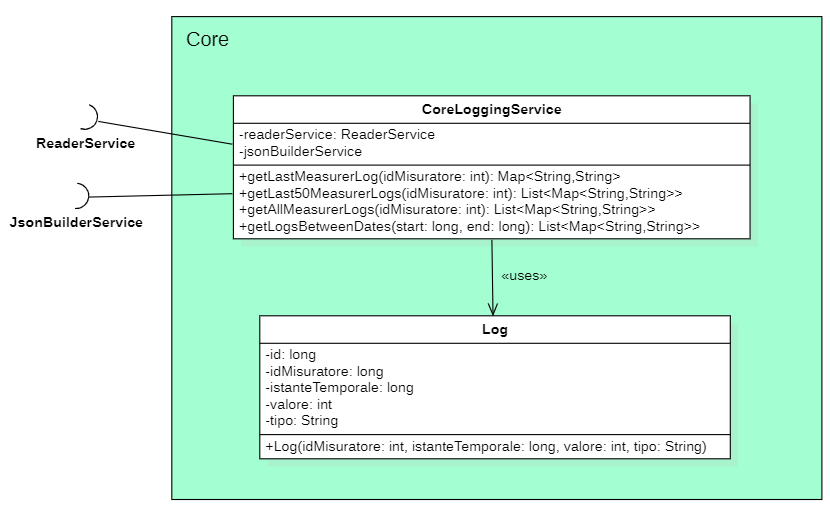
\includegraphics[width=0.6\textwidth]{img/classi_logging.png}
    \caption{Vista generale del sistema di logging}
    \label{fig:general_logging}
\end{figure}

\section{Repository}
Il LogRepository è un'interfaccia repository jpa ed esegue fisicaente le operazioni sul database.

\section{Servizi}

I servizi sono in generale le interfaccie ad alto livello delle funzionalità del sistema. Sono composti da classi che si occupano di gestire le richieste e di fornire i dati richiesti.

\subsection{ReaderService}
ReaderService si occupa di leggere e fornire i dati dei log dal database in base alla richiesta.

ReaderService viene realizzata in localReaderService per i test. Invece per connettersi al db viene utilizzata la classe DatabaseReaderService.

\section{Core}
Il core è il nucleo del sistema ed in generale si pone come facade per tutti i servizi che si trovano all'interno del microservizio. Questa classe si occupa di gestire le richieste e di fornire i dati richiesti.
Principalmente questa classe viene utilizzata dall'interfaccia REST.

\section{Log}
La classe Log viene utilizzata per trasferire le informazioni tra le varie classi ed è costruito da logrepository quando fa operazioni sul database e deve ritornarne uno.

\section{JsonBuilderService}
Si occupa di creare i json da ritornare all'interfaccia rest a partire dai log.

\section{ Config}
La classe Cofig genera i bean che servono alle altre classi per funzionare.



\section{Interfaccia REST}

\begin{figure}[ht]
    \centering
    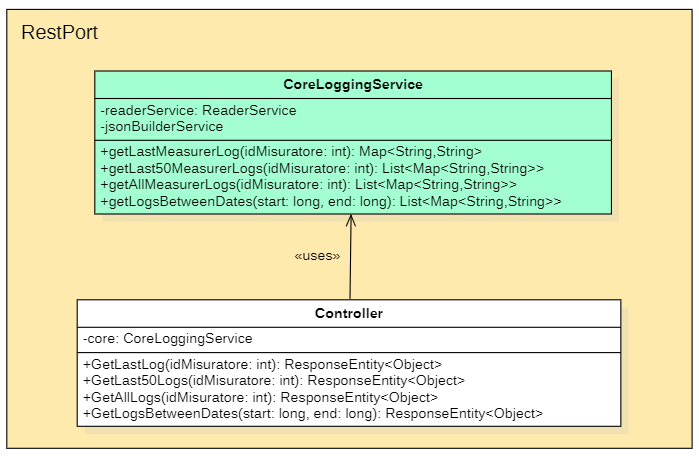
\includegraphics[width=0.8\textwidth]{img/classi_logging_port_rest.png}
    \caption{Vista generale del sistema di logging}
    \label{fig:general_logging}
\end{figure}


